\notechapter{N-20251009}{Latent Variable Models: Priors, Decoders, and Intractable Posteriors}

\section{From autoencoders to latent variable models}

A deterministic autoencoder is a pair of maps
\[
  x\xrightarrow{\mathrm{encoder}}h\xrightarrow{\mathrm{decoder}}\widehat x.
\]
The code \(h\) is a deterministic representation of \(x\).  A VAE keeps the encoder--decoder visual shape, but the mathematical object is different.  The hidden representation is a random variable \(Z\), and the decoder defines a conditional distribution, not merely a reconstruction function.

The generative story is
\[
  z\sim p(z),\qquad x\sim p_\theta(x\mid z).
\]
Thus a VAE is best understood as a latent variable model equipped with an efficient approximate inference model.

The key distinction is:
\[
\begin{array}{c|c}
\text{deterministic autoencoder} & \text{VAE / latent variable model}\\
\hline
h=f_\phi(x) & z\sim q_\phi(z\mid x)\\
\widehat x=g_\theta(h) & x\sim p_\theta(x\mid z)\\
\text{reconstruction map} & \text{probabilistic generative model}
\end{array}
\]

\section{The generative story}

The model begins with a prior distribution on the latent variable:
\[
  p(z).
\]
In the basic VAE,
\[
  p(z)=\mathcal N(0,I).
\]
This prior says that latent variables should live in a simple, continuous, isotropic space.

Given \(z\), the decoder defines the likelihood of an observation:
\[
  p_\theta(x\mid z).
\]
The joint density is then
\[
  p_\theta(x,z)=p(z)p_\theta(x\mid z).
\]
This formula is the mathematical core of the generative model.

The decoder network does not directly output a final sample.  It outputs parameters of a distribution.  For binary data, one often writes
\[
  p_\theta(x\mid z)=\operatorname{Bernoulli}(x;\pi_\theta(z)).
\]
Here \(\pi_\theta(z)\) gives the success probabilities of the Bernoulli coordinates.  For real-valued data, one may use
\[
  p_\theta(x\mid z)=\mathcal N(x;\mu_\theta(z),\sigma^2 I).
\]
Here the decoder outputs a mean \(\mu_\theta(z)\), and the variance is either fixed or parameterized separately.

\section{Graphical model notation}

The generative model has one directed probabilistic arrow:
\[
  z\longrightarrow x.
\]
A small diagram is:

\begin{center}
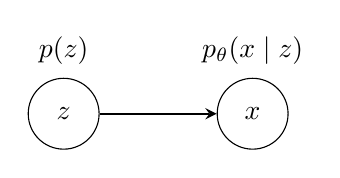
\begin{tikzpicture}[>=stealth,node distance=2.4cm]
  \node[draw,circle,minimum size=0.9cm] (z) {$z$};
  \node[draw,circle,minimum size=0.9cm,right of=z] (x) {$x$};
  \draw[->,thick] (z) -- (x);
  \node[above of=z,node distance=0.8cm] {$p(z)$};
  \node[above of=x,node distance=0.8cm] {$p_\theta(x\mid z)$};
\end{tikzpicture}
\end{center}

For a dataset \(x^{(1)},\ldots,x^{(N)}\), the story repeats independently:
\[
  z^{(i)}\sim p(z),\qquad x^{(i)}\sim p_\theta(x\mid z^{(i)}).
\]
The parameters \(\theta\) are shared across all observations.

\section{Marginal likelihood}

The model likelihood of one observation is obtained by integrating out the latent variable:
\[
  p_\theta(x)=\int p_\theta(x,z)\,dz
  =\int p(z)p_\theta(x\mid z)\,dz.
\]
For a dataset, maximum likelihood would choose \(\theta\) by maximizing
\[
  \sum_{i=1}^N \log p_\theta(x^{(i)}).
\]
Equivalently, one wants the model distribution \(p_\theta(x)\) to assign high probability density to the observed data.

The problem is that the integral
\[
  \int p(z)p_\theta(x\mid z)\,dz
\]
is usually intractable.  If \(p_\theta(x\mid z)\) is parameterized by a nonlinear neural network, there is no closed-form expression for the integral over \(z\).

This is the first reason variational methods enter.

\section{The posterior problem}

The posterior distribution of the latent variable is
\[
  p_\theta(z\mid x)=\frac{p_\theta(x,z)}{p_\theta(x)}
  =\frac{p(z)p_\theta(x\mid z)}{\int p(z')p_\theta(x\mid z')\,dz'}.
\]
The numerator is easy to evaluate up to normalization.  The denominator is the marginal likelihood, which is the same difficult integral.

Therefore the model has a basic asymmetry:
\[
\begin{array}{c|c}
\text{sampling direction} & \text{inference direction}\\
\hline
z\sim p(z),\;x\sim p_\theta(x\mid z) & p_\theta(z\mid x)\text{ is hard}
\end{array}
\]

This is the central probabilistic problem behind VAEs:
\[
\begin{array}{c}
  \text{to train the model, we want }\log p_\theta(x),\\
  \text{to understand }\log p_\theta(x),\text{ we need to reason about }z,\\
  \text{but the true posterior }p_\theta(z\mid x)\text{ is intractable.}
\end{array}
\]

\section{Why naive Monte Carlo is not enough}

One might try to estimate the marginal likelihood by drawing samples from the prior:
\[
  z^{(\ell)}\sim p(z),\qquad
  p_\theta(x)\approx\frac1L\sum_{\ell=1}^L p_\theta(x\mid z^{(\ell)}).
\]
This is formally reasonable, but in high dimension it is usually inefficient.  Most prior samples \(z\) do not explain a fixed observation \(x\) well.  The average is then dominated by rare samples that land in useful regions of latent space.

For inference about a particular \(x\), we would rather sample \(z\) values that are already plausible explanations of \(x\).  That is the motivation for introducing an approximate posterior.

\section{The recognition model}

A VAE introduces a family
\[
  q_\phi(z\mid x)
\]
to approximate the true posterior \(p_\theta(z\mid x)\).  This is often called the recognition model or encoder.

The standard Gaussian encoder has the form
\[
  q_\phi(z\mid x)=\mathcal N(z;\mu_\phi(x),\operatorname{diag}(\sigma_\phi^2(x))).
\]
The functions \(\mu_\phi(x)\) and \(\sigma_\phi(x)\) are outputs of a neural network.  Mathematically, they parameterize a distribution over latent variables.

It is important not to confuse the two conditional distributions:
\[
\begin{array}{c|c|c}
\text{symbol} & \text{name} & \text{direction}\\
\hline
p_\theta(x\mid z) & \text{decoder likelihood} & z\to x\\
q_\phi(z\mid x) & \text{approximate posterior / encoder} & x\to z
\end{array}
\]
Only \(p_\theta(x\mid z)\) belongs to the generative model.  The encoder \(q_\phi(z\mid x)\) is introduced to make inference and training feasible.

\section{Amortized inference}

Classical variational inference might introduce separate variational parameters for each data point.  For example, for every observation \(x^{(i)}\), one could choose its own mean and variance:
\[
  q_i(z)=\mathcal N(z;\mu_i,\operatorname{diag}(\sigma_i^2)).
\]
A VAE instead uses one shared inference network:
\[
  x\longmapsto \mu_\phi(x),\qquad x\longmapsto \sigma_\phi(x).
\]
This is called amortized inference.  The cost of inference is amortized across the dataset: after learning \(\phi\), the model can quickly produce an approximate posterior for a new \(x\).

The mathematical tradeoff is that the family is restricted.  We do not choose arbitrary variational parameters for each observation; we require them to be outputs of the same function.

\section{The VAE model diagram}

The two directions can be displayed together:

\begin{center}
\begin{tikzpicture}[>=stealth,node distance=3.0cm]
  \node[draw,circle,minimum size=0.9cm] (z) {$z$};
  \node[draw,circle,minimum size=0.9cm,right of=z] (x) {$x$};
  \draw[->,thick] (z) -- node[fill=white,inner sep=1pt,above] {$p_\theta(x\mid z)$} (x);
  \draw[->,thick,bend left=38] (x) to
    node[fill=white,inner sep=1pt,below=2pt] {$q_\phi(z\mid x)$} (z);
  \node at ($(z)+(0,-1.35)$) {latent};
  \node at ($(x)+(0,-1.35)$) {observed};
\end{tikzpicture}
\end{center}

The upper arrow is the probabilistic generative story.  The lower arrow is the learned inference shortcut.  The VAE objective will force these two directions to be compatible, but they play different roles.

\section{Remaining derivation}

At this point, the problem is clear.  We want to maximize
\[
  \log p_\theta(x),
\]
but
\[
  p_\theta(x)=\int p(z)p_\theta(x\mid z)\,dz
\]
is hard.  We also want to use
\[
  p_\theta(z\mid x),
\]
but it contains the same intractable marginal likelihood.

The solution is to introduce \(q_\phi(z\mid x)\), then build a lower bound on \(\log p_\theta(x)\) that can be optimized.  That lower bound is the evidence lower bound, or ELBO.

The next note derives it from two facts:
\[
  D_{\mathrm{KL}}(q\Vert p)\ge0,
  \qquad
  \log\mathbb E[Y]\ge\mathbb E[\log Y].
\]
